\documentclass[14pt]{extarticle}
\usepackage[utf8]{inputenc}
\usepackage[spanish]{babel}
\usepackage{enumerate}
\usepackage{graphicx}
\usepackage{listings}
\usepackage{dsfont}
\usepackage{caption}
\usepackage{subfigure}
\usepackage{ amssymb }
\usepackage{amsthm}
\usepackage{pdflscape}
\usepackage{ marvosym }
\usepackage{amsmath}
\usepackage{ mathrsfs }
\usepackage{hyperref}

\title{Ingeniería Informática: \\
	\textbf{Inteligencia del negocio.}}
\author{Alberto Argente del Castillo Garrido. \\
	aargente@correo.ugr.es}
\date{\today.}
\begin{document}
\maketitle
\tableofcontents

\newpage
\section{Introducción}
En esta usaremos métodos para el aprendizaje supervisado en regresión sobre una competición de la plataforma Kaggle, en concreto la competición será House Prices: Advanced Regression Techniques (https://www.kaggle.com/c/house-prices-advanced-regression-techniques) cuyo objetivo es el de predecir el precio final de una vivienda a partir de 79 variables que describen diferentes aspectos de ella. Para ello contamos con datos reales recogidos entre 2006 y 2010. \\

Respecto a mi nombre en Kaggle, será Alberto Argente (UGR).

\section{Resolución de la práctica}
En esta sección documentaré el trabajo realizado durante la práctica, el cual contedrá un tabla con la siguiente información:
\begin{itemize}
	\item Fecha y hora de la subida a Kaggle.
	\item Posición ocupada en ese momento.
	\item Score al subir el script a Kaggle.
	\item RMSLE sobre los datos de entrenamiento.
	\item Breve descripción del preprocesado realizado.
	\item Breve descripción de los algoritmos de regresión empleados.
	\item Configuración de parámetros de los algoritmos.
\end{itemize}

Dado que la configuración de los algoritmos y el preprocesado ocupan más espacio del que podría llegar a usar en la tabla, voy a detallar tras la tabla con los resultados el preprocesado para las subidas. A continuación, tablas \ref{ress1} y \ref{ress2} se muestran los resultados obtenidos: \\

\begin{table}[h!]
	\centering
	\caption{Tabla de resultados 1}
	\label{ress1}
	\hspace*{-1.5cm}
	\begin{tabular}{|c|c|c|c|c|c|c|}
		\hline
		\textbf{Subida} & \textbf{Fecha} & \textbf{Hora} & \textbf{Score} & \textbf{RMSLE train} & \textbf{Algoritmos}                                            & \textbf{Posición} \\ \hline
		1º              & 26/12/17       & 22:02         & 0.12197        & 0.1079684            & Xgboost                                                        & 763               \\ \hline
		2º              & 26/12/17       & 22:13         & 0.12298        & 0.1071981            & Xgboost                                                        & 763               \\ \hline
		3º              & 26/12/17       & 22:29         & 0.12298        & 0.1094292            & Xgboost                                                        & 763               \\ \hline
		4º              & 27/12/17       & 17:51         & 0.12160        & 0.09603789           & \begin{tabular}[c]{@{}c@{}}Ensamble\\ XgbGbm\end{tabular}      & 753               \\ \hline
		5º              & 28/12/17       & 20:56         & 0.11988        & 0.1106704            & \begin{tabular}[c]{@{}c@{}}Ensamble\\ XgbGbmLasso\end{tabular} & 576               \\ \hline
		6º              & 29/12/17       & 13:46         & 0.11952        & 0.1111768            & \begin{tabular}[c]{@{}c@{}}Ensamble\\ XgbGbmLasso\end{tabular} & 550               \\ \hline
		7º              & 30/12/17       & 21.54         & 0.12850        & 0.1095923            & \begin{tabular}[c]{@{}c@{}}Ensamble\\ XgbGbmLasso\end{tabular} & 559               \\ \hline
		8º              & 2/1/18         & 18:59         & 0.12338        & 0.1111022            & \begin{tabular}[c]{@{}c@{}}Ensamble\\ XgbGbmLasso\end{tabular} & 572               \\ \hline
		9º              & 3/1/18         & 11:30         & 0.11955        & 0.1144636            & \begin{tabular}[c]{@{}c@{}}Ensamble\\ XgbGbmLasso\end{tabular} & 574               \\ \hline
		10º             & 4/1/18         & 17:28         & 0.11969        & 0.0900812            & \begin{tabular}[c]{@{}c@{}}Ensamble\\ XgbGbmLasso\end{tabular} & 611               \\ \hline
		11º             & 4/1/18         & 18:40         & 0.11920        & 0.1011002            & \begin{tabular}[c]{@{}c@{}}Ensamble\\ XgbGbmLasso\end{tabular} & 594               \\ \hline
		12º             & 4/1/18         & 23:47         & 0.11916        & 0.103465             & \begin{tabular}[c]{@{}c@{}}Ensamble\\ XgbGbmLasso\end{tabular} & 592               \\ \hline
		13º             & 4/1/18         & 23:50         & 0.11888        & 0.1013893            & \begin{tabular}[c]{@{}c@{}}Ensamble\\ XgbGbmLasso\end{tabular} & 578               \\ \hline
		14º             & 4/1/18         & 23:52         & 0.11869        & 0.09846604           & \begin{tabular}[c]{@{}c@{}}Ensamble\\ XgbGbmLasso\end{tabular} & 567               \\ \hline
	\end{tabular}
\end{table}

\begin{table}[h!]
	\centering
	\caption{Tabla de resultados 2}
	\label{ress2}
	\hspace*{-1.5cm}
	\begin{tabular}{|c|c|c|c|c|c|c|}
		\hline
		\textbf{Subida} & \textbf{Fecha} & \textbf{Hora} & \textbf{Score} & \textbf{RMSLE train} & \textbf{Algoritmos}                                            & \textbf{Posición} \\ \hline
		15º             & 4/1/18         & 23:55         & 0.11890        & 0.09803138           & \begin{tabular}[c]{@{}c@{}}Ensamble\\ XgbGbmLasso\end{tabular} & 567               \\ \hline
		16º             & 4/1/18         & 23:57         & 0.11862        & 0.09840978           & \begin{tabular}[c]{@{}c@{}}Ensamble\\ XgbGbmLasso\end{tabular} & 561               \\ \hline
		17º             & 4/1/18       & 23:59         & 0.11883        & 0.09919482           & \begin{tabular}[c]{@{}c@{}}Ensamble\\ XgbGbmLasso\end{tabular} & 561               \\ \hline
	\end{tabular}
\end{table}

\subsection{Subidas 1,2,3}

He juntado estas 3 subidas ya que el preprocesado es igual y sólo cambié algún parámetro del algoritmo utilizado, en este caso Xgboost únicamente. Para el preprocesado, lo primero que hice fue eliminar outliers de la variable GrLivArea, la cual es la variable que más correlación tiene con la variable SalePrice, figura \ref{im1}. \\

\begin{figure}[h!]
	\centering
	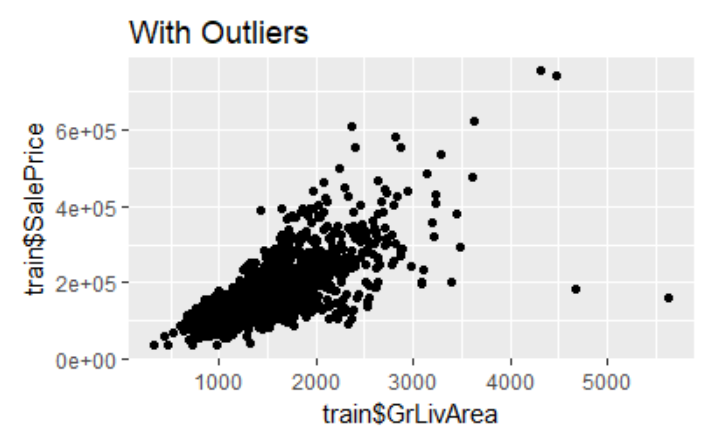
\includegraphics[width=11cm]{img/outliers.png}
	\caption{Outliers en GrLivArea}
	\label{im1}
\end{figure}


Una vez eliminados los outliers lo que he hecho ha sido normalizar el valor de SalePrice, para ello he aplicado el logaritmo a la variable SalePrice quedando como se refleja en la figura \ref{im2}

\begin{figure}[h!]
	\centering
	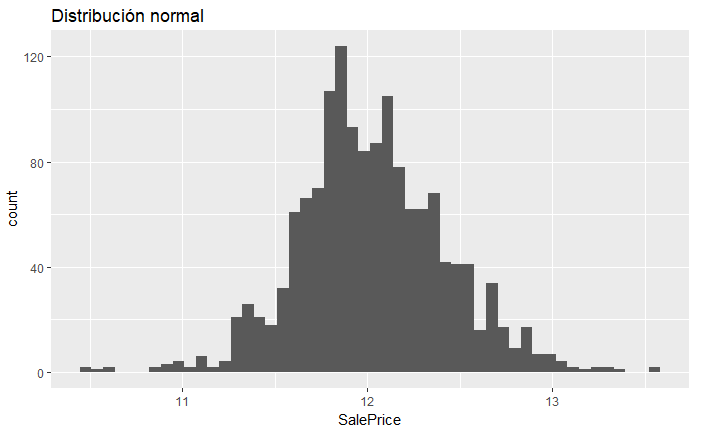
\includegraphics[width=10cm]{img/SalePriceNormalice.png}
	\caption{Valores perdidos previos a la imputación.}
	\label{im2}
\end{figure}

Tras ello lo que he hecho ha sido eliminar los valores perdidos tanto de train como de test. Como se puede ver en la imagen \ref{im3} el número de valores perdidos es muy alto para algunas variales, como puede ser el caso de PoolQC, Al leer el data\_descripcion proporcionado por kaggle, vi que para muchas variables el valor NA no significa que no se sepa el valor, sino que no hay nada en esa casa, por ejemplo en la variable PoolQC, el valoro que aparece como NA significa "No pool", por tanto cambio el valor "NA" por "None" para así eliminar todos estos valores perdidos y saber cuáles quedan. \\	


\begin{figure}[h!]
	\centering
	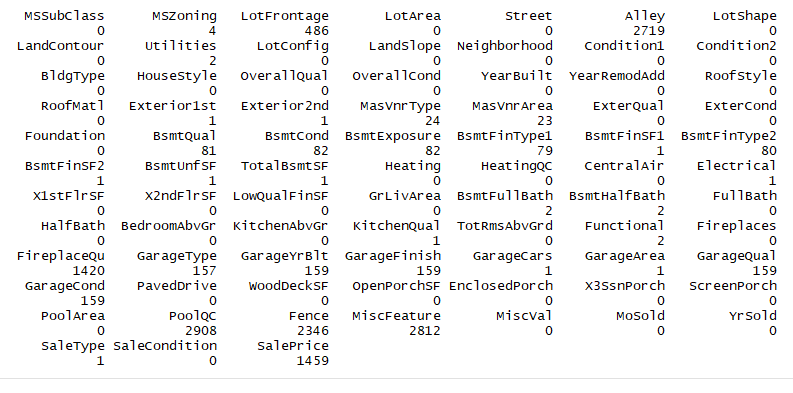
\includegraphics[width=15cm]{img/fullna.png}
	\caption{Valores perdidos previos a la imputación de datos.}
	\label{im3}
\end{figure}



Para el resto de variables que tienen valor NA, lo que hice para los valores numéricos es calcular la media, y para las atributos categóricos calcular la moda. Además elimino el atributo "Utilities" dado que no tiene variabilidad dentro del data set no aportará mucho, quedando así sin valores perdidos salvo los del conjunto de test \ref{im4}. \\

\begin{figure}[h!]
	\centering
	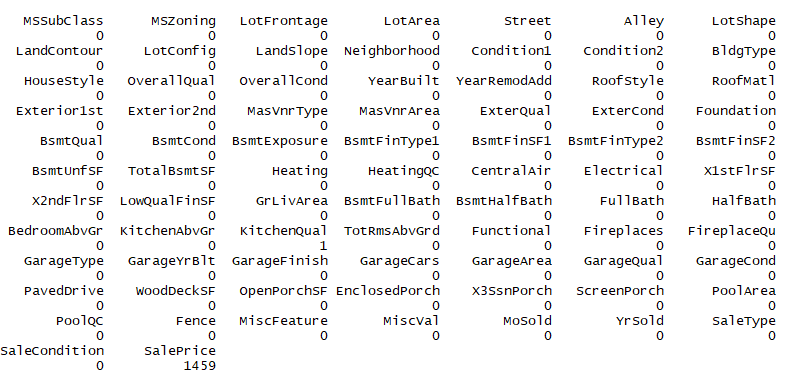
\includegraphics[width=15cm]{img/zerona.png}
	\caption{Valores perdidos tras la imputación de datos..}
	\label{im4}
\end{figure}

Una vez eliminé los valores perdidos lo que he hecho ha sido poner como caracter algunas variables numéricas, ya que el valor numérico o bien quiere decir otra cosa como puede ser el caso de MsSubClass, o bien representan un año, como es YrSold. \\

Una vez hecho esto procedo a binarizar los atributos categóricas, para así poder utilizar bien los algoritmos que voy a utilizar, quedando así un total de 221 atributos. \\

Por último apliqué sobre aquellas variables que tengan la curtosis mayor de 0.75 la transformación BoxCox la cual corrige sesgos en la distribución de errores, varianzas desiguales y mejorar la correlación entre las variables. \\

Una vez hecho esto preparo la partición 70-20 para training-test, para así entrenar el modelo, para ello he utilizado Xgboost. Para los parámetros de Xgboost, utilicé la función xgb.cv la cual usa Xgboost con Cross Validation, para así poder observar cómo decrece el RMSE y el número de iteraciones hasta así obtener unos parámetros que me dieran mejor o peor resultados. La lista de parámetros que le paso es: "objetive: reg-linear" para indicarle que es un problema de regresión, "eval-metric = rmse" para indicarle qué medida queremos calcular, "nthread = 4" para que use 4 hebras en la ejecución, "eta = 0.01" (learning-rate), "gamma = 0.01", "max\_depth = 6", min\_child\_weight = 0.178171", "subsample = 0.5213", "colsample\_bytree = 0.484". \\

El parámetro que varía entre las 3 subidas es "max\_depth", el cual en la subida 1 fue de 6, en la subida 2 fue 10 y en la tercera subida fue 7. El cambio se debió a que usando 10 como max\_depth obtune un rmse parecido y algo más alto lo que podía indicar que quizás no tuviera tanto sobreajuste. \\


\subsection{Subida 4}
En la cuarta subida dejo igual todo el preprocesado anterior sólo que he añadido al algoritmo Gradient Boosting para posteriormente hacer un ensamble de ambos modelos, ya que Xgboost al ser más potente que otros algoritmos puede generar algo de sobreaprendizaje en el modelo, por lo que si añadimos otro algoritmo que no obtenga tan buenos resultados en train para así poder tener un ensamble con el que obtener mejores resultados. \\

Tras realizar pruebas ejecutando Gradient Boosting (GBM), los parámetros con los que decidí ejecutar el algoritmo son: "shrinkage = 0.01", "interaction.depth = 3", "bag.fraction = 0.5", "n.minobsinnode = 10", "cv.foldds = 5", "distribution = 3", "n.trees = 3000".  \\

Una vez tenemos los resultados de gbm y de xgboost, lo que hago es haber un ensamble dándole la misma importancia tanto a Xgboost como a GBM. \\

\subsection{Subidas 5 y 6}
Para la quinta y la sexta subida he añadido Lasso como algoritmo para entrenar el modelo, para así tener un mejor ensamble al añadir otro modelo más y que tenga un funcionamiento distinto al que tienen Xgboost y Gradient Boosting, para así intentar obtener una mejora mayor.  \\

Para Lasso he aprovechado el paquete de gmlnet que me permite usar Cross Validation y la configuración usada con Lasso ha sido la siguiente: "family = gaussian", "alpha = 0.1655" y "nfolds = 5".

Para la quinta subida el ensamble realizado ha sido darle 0.3 a Xgboost, 0.4 a GBM y 0.3 a Lasso, mientras que en la sexta subida le di a Xgboost 0.4, a GBM 0.3 y a Lasso 0.3. \\

\subsection{Subida 7}

En este caso he intentado preprocesado de forma distinta a como lo hacía en las subidas anteriores, para ello par ala imputación de datos en vez de hacerlo de forma manual he utilizado un Random Forest, ya que estuve comparando entre K-nn y Random Forest y obtuve mejores resultados con Random Forest. \\

Aún así había algunas variables las cuales no eliminaban sus valores perdidos, como se puede ver en la figura \ref{im5}, con cualquier algoritmo utilizado con el paquete Mice de R, por tanto fijándome en los que quedaban como NA, los imputé aplicando la media en caso de que fueran numéricas, o en la moda si son categóricas. \\

\begin{figure}[h!]
	\centering
	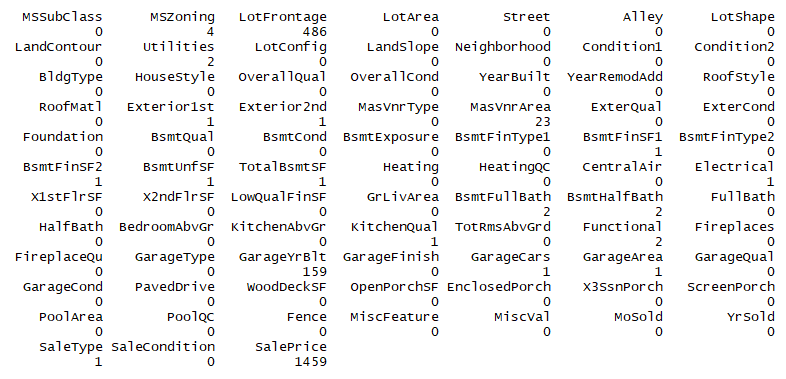
\includegraphics[width=15cm]{img/nassecpre.png}
	\caption{Valores perdidos tras la imputación de datos con Random Forest.}
	\label{im5}
\end{figure}

Una vez realizada la imputación de datos lo que hice fue binarizar las variables categorícas y aplicar la transformación BoxCox a aquellas variables que tuvieran una Curtosis mayor de 0.75. \\

Al tener tantas variables pensé en aplicar selección de características para así quedarme con menos variables pero que representaran mejor el problema, para ello usé como algoritmo Boruta. \\

Tras aplicar Boruta utilicé las mismas configuraciones con los algoritmos utilizados, Gradient Boosting, Xgboost y Lasso, que las utilizada anteriormente y subí aquella subida que mejor resultado me dio in-train, 0.4 para Xgboost, 0.4 para Gradient Boosting y 0.2 para Lasso. \\

\subsection{Subida 8}

En esta subida lo que hice fue añadir las variables categóricas que quería binarizar, ya que en la subida 7 pensé que lo había hecho pero al revisar el código vi que no, por tanto esta vez tras aplicar Boruta me queda con tan solo 84 variables, de 221 que tenía originalmente en las primeras subidas, y por tanto esperaba tener una mejora sustancial ya que muchas de las variables que obtenía antes no llegaban a ser importantes.

Este cambió mejoró mucho con respecto a la subida anterior, pero siguió sin ser una mejora respecto a mi mejor subida.

\subsection{Subida 9}

Dado que no mejoró el anterior preprocesamiento decidí volver al primero pero siguiendo cambiando los parámetros de los algoritmos.

En el caso de Gradient Boosting, cambié shrinkage a 0.01 a 0.015, ya que estuve haciendo diferentes pruebas y conseguía obtener mejores resultados, cambié el bag.fraction de 0.5 a 0.5308 y n.tress de 3000 a 2000 ya que aunque yo indicara que usara 3000 no llegaba a pasar de 2000 y convergía, por lo que no era necesario que tuviera tanto y usando 2000 el resultado seguía siendo mejor que poniendo 3000 pese a no llegar a los 2000 árboles.

Para Lasso cambié el alpha de 0.1655 a 0.9955, obteniendo en este caso mejoras respecto al anterior.

Y por último para Xgboost usé un eta de 0.05, cambié max\_depth de 6 a 3, y añadí algunos parámetros adicionales que estuve consultando en el manual de Xgboost, que son silent que le di de valor 1, alpha = 0.4640 y gamma = 0.8574.


Pese a que estos resultados que obtenía eran mejores, el resultado que llegaba a obtener con Gradient Boosting eran parecidos a Xgboost, por lo tanto decidí no usarlo dado que pensé que podía tener un sobreaprendizaje parecido a Xgboost por tanto decidí hacer un ensamble de Xgboost y de Lasso, dándole a Xgboost 0.55 y a Lasso 0.45.

\subsection{Subidas 10 y 11}

En esta subida en matenido la imputación de datos igual que en las primeras subidas, y he binarizado las variables categóricas, pero en este caso para las variables numéricas no he aplicado las transformación BoxCox, en este caso he aplicado el logaritmo, al igual que a la variable SalePrice, para así normalizar los valores e intentar tener una mejor correlación de estas variables con SalePrice. \\

Para esta subida he hecho un ensamble de GBM, Lasso y Xgboost, manteniendo los mismos para GBM. Para Lasso cambié el alpha a 0.0155 y para Xgboost cambié el valor de eta (learning rate) a 0.01, gamma = 0.0, y subsample = 0.2. \\

Tras esto los pesos asignados para la subida 10 son 0.4 a Xgboost, 0.3 a GBM y 0.3 a Lasso.\\

Para la subida 11 dejé todos los parámetros iguales y cambié los pesos asignados a los modelos, dando 0.5 a Xgboost, 0.25 a GBM y 0.25 a Lasso.\\

\subsection{Subida 12}

Para esta subida creé un nuevo preprocesamiento, en este creé una función que se llama comb\_num, la cual recibe como parámetro un dataframe y genera uno nuevo, no sólo con las mismas variables sino que además generamos nuevas variables. \\

Para ello en esta función a parte de las variables de las que partimos en el problema, creamos las siguientes variables nuevas:

\begin{itemize}
	\item Remodeled: Año en el que fue remodelada
	\item RecentModel: Aquellas que han sido remodeladas el mismo año que fueron vendidas.
	\item NewHouse: Casas que fueron vendidas el mismo año que fueron construidas.
	\item HasOpenPorch: Casas que tenían un porche al descubierto.
	\item HasEnclosedPorch: Casas que tenían un porche cubierto.
	\item Has3SsnPorch: Casas que tienen un porche en la 3º planta.
	\item TotalArea1st2nd: Suma del área de las plantas 1 y 2.
	\item YearSinceRemodel: Años que han pasado desde que fue remodelada. 
\end{itemize}


Tras esto elimino los valores perdidos al igual que hacía en las primeras subidas, es decir, para algunas variables cuyos valores NA no representaban realmente NA lo cambiaba por None, para las numéricas les ponía 0, y para las categóricas les ponía la moda. \\


Esta vez para las variables numéricas probé inTrain usar tanto la transformación BoxCox como aplicar al logaritmo, pero los resultados aplicados con BoxCox eran mejores que aplicando el logaritmo, por tanto apliqué BoxCox.\\

Una vez hecho esto aplico los algoritmos que he estado aplicando, GBM, Lasso y Xgboost. Para Gradient Boosting los parámetros son: shinkage = 0.07, interaction.depth = 3, bag.fraction = 0.5308, m.minibsnode = 10, cv.folds = 5, distribution = gaussian y n.trees = 3.

Para Lasso los parámetros son: nfolds = 5, family = gaussian, alpha = 0.00099. Y por último para Xgboost los parámetros son: nrounds = 7, objetive = reg:linear, eval\_metric = rmse, nthreadh = 4, eta = 0.01, gamma = 0.0, max\_depth = 3, min\_child\_weight = 1.78171, subsample = 0.2, colsample\_bytree = 0.2, silent = 1, alpha = 0.4645, lambda = 0.6, random\_state = 123.

Una vez tengo los modelos hago un Ensamble de ellos con los siguientes pesos: 0.75 Xgboost, 0.1 GBM, 0.15 Lasso.

\subsection{Subidas 13, 14}

Para la subida 13 he mantenido el mismo preprocesamiento que en la subida 12, solo que el cambio realizado ha sido sobre los parámetros de Gradient Boosting, para los cuales los parámetros utilizados han sido: shrinkage = 0.07, interaction.depth = 3, bag.fraction = 0.5308, n.minobsinnode = 15, cv.folds = 5, distribution = gaussian, n.trees = 3000.

Con esto se obtienen mejoras inTrain tanto en Gradient Boosting como en el ensamble y en este caso las ponderaciones realizadas han sido parecidas a la anterior: 0.7 Xgboost, 0.15 Lasso y 0.15 Gradient Boosting 

Para la subida 14 he mantenido solo he cambiado el parámetro de Gradient Boosting n.minonsinnode de 15 a 10, de forma que también seguía obteniendo una mejora in train, por tanto manteniendo las mismas ponderaciones que antes, 0.7 Xgboost, 0.15 Lasso y 0.15 Gradient Boosting.


\subsection{Subidas 15, 16 y 17}

Las tres últimas subidas son cambios en las ponderaciones de la subida 13, teniendo en la subida 15 las ponderaciones: 0.7 para Xgboost, 0.2 para Lasso y 0.1 para Gradient Boosting. \\

Para la subida 16 las ponderaciones usadas han sido erróneas, aunque no me di cuenta a la hora de subirlo porque la hora de finalización estaba cercana, era de 0.75 Xgboost, 0.15 Lasso y 0.15 Gradient Boosting. Pese a eso la subida fue la mejor subida a Kaggle que he subido. \\

Para la última subida cambié los parámetros para intentar darle menos importancia a Xgboost, de forma que quedaron: 0.3 Xgboost, 0.2 Lasso y 0.5 Gradient Boosting. \\


\section{Ideas no realizadas}

He añadido esta sección para comentar algunas ideas que pensé realizar pero que no he podido realizar. \\

La primera idea que tuve fue hacer un stacked-model, de forma que utilizaba varios algoritmos para entrenar cada uno un modelo, y usando los resultados de estos modelos entranaba un modelo nuevo, para ello estuve intentado realizarlo con el paquete de Caret, pero tuve algunos errores al intentar hacerlo funcionar y preferí intentar otras cosas porque no sabia bien el funcionamiento que podía tener. La idea era usar Xgboost, Gradient Boosting, Lasso, Elastic-Net y una red neuronal, pero como inconveniente tenía que no podía utilizar tantos parámetros como en los paquetes individuales, y además el modelo a entrar con los resultados de los algoritmos nombrados anteriormente era Random Forest, ya que usar otra vez Gradient Boosting o Lasso creo que podría haber creado más sobreajuste. \\

La otra idea que intenté llevar a cabo pero finalmente no realicé, fue eliminar más outliers pero de todas las variables, ya que en mi caso sólo eliminaba de una, aplicando un algoritmo, pero el único algoritmo que utilicé no me eliminó ninguna instancia, cosa que el algoritmo estaba mal implementado, y por tanto como la entrega estaba cercana decidí hacer otro tipo de preprocesamiento. \\


\section{Referencias}

Para esta práctica me he fijado en muchos tutoriales de visualización que he encontrado en Kaggle ya que tuve problemas a la hora de generar algunas gráficas, y con ellos me ayudé a ver la correlación entre algunas variables con SalePrice.

Para el uso de Boruta utilicé la documentación oficial de R, al igual que con Mice.

\end{document}
